\section{(3) Asynchronous communication models overview}
\label{sec:com_models_overview}

In synchronous communication, send and receive events are essentially viewed as a single entity, i.e. a receive event always happens simultaneously with its corresponding send event. The whole idea behind (fully) asynchronous communication is to decouple send and receive events, so that a receive event can happen indefinitely after its corresponding send event. However, by introducing some additional contraints on asynchronous communication, we can obtain new communication models that sit somewhere between synchronous and fully asynchronous communication. These kind of communication models are often used interchangably in literature and generally referred to as "asynchronous", without providing a clear definition. In this section, we will present 7 different asynchronous communication models, which were already introduced in \cite{DBLP:journals/fac/ChevrouHQ16} (even though they do not consider unmatched messages). A major difference is that in \cite{DBLP:journals/fac/ChevrouHQ16} these communication models are addressed from a linearizations standpoint, whereas we are interested in MSCs. Recall that a single MSC can have several possible linearizations. The work in \cite{DBLP:journals/fac/ChevrouHQ16} describes the properties that a single linearization must satisfy in order to be realizable by a system that uses a given communication model. On the other hand, we are interested in understanding if a given MSC describes a computation that can be realized by a system that uses some communication model $CM$. In other words, given a MSC we want to know if it has at least one linearization that respects the constraints imposed by $CM$. If that is the case, the MSC represents a behaviour that can be exhibited by a system that uses $CM$ as a communication model. These are two fundamentally dissimilar problems; at the end of this section we provide an example to clarify the difference. In our work, we are going to formally characterize the classes of MSCs which represent valid computations for all of these 7 asynchronous communication model. We also show how these classes form a well-defined hierarchy, which does not correspond entirely to that found in \cite{DBLP:journals/fac/ChevrouHQ16}.

We model a distributed system as a set of concurrent Finite-State Machines (FSMs) that exchange messages asynchronously through channels. Each FSM models a single machine/process of the system and transitions are labeled with "send" and "receive" operations, which specify the sender and the receiver of a message. In our work we consider only point-to-point communication, that is, messages that have exactly one sender and one receiver. The role of the communication model is to impose an order on the reception of messages, according to its specification. For instance, the delivery of a message could be delayed or even prevented by a communication model $CM$, so as to ensure that messages are received in an order that is valid for $CM$. The 7 communication models that we address all impose different constraints on the order in which messages can be received.

\subsection{Fully asynchronous}
In the fully asychronous communication model (or simply asynchronous) messages can be received at any time once they have been sent. In asynchronous communication, send events are non-blocking, i.e. the sender of a message does not have to wait for it to be delivered to the recipient, in order to resume normal operations. Fig.~\ref{fig:fully_asy_ex} shows a computation that can be executed by a system that uses asynchronous communication; indeed, even if $m_1$ is sent before $m_2$, $q$ does not have to receive $m_1$ first. For convenience, we will refer to a system that uses asynchronous communication simply as an asynchronous system. In a similar way, an MSC such that in Fig.~\ref{fig:fully_asy_ex} will be referred to as an asynchronous MSC, since it represents a computation that is realizable by an asynchronous system. The same jargon will also be used for all the other communication models. We will call $\asMSCs$ the set of all asynchronous MSCs.

\begin{figure}[h]
	\begin{center}
		\begin{tikzpicture}
			\newproc{0}{p}{-2};
			\newproc{2}{q}{-2};	
		
			\newmsgm{0}{2}{-0.5}{-1.7}{1}{0.1}{black};
			\newmsgm{0}{2}{-1.7}{-0.5}{2}{0.25}{black};
				
			\end{tikzpicture}
		\caption{An asynchronous MSC.}
		\label{fig:fully_asy_ex}
	\end{center}
\end{figure}

\subsection{FIFO $\oneone$ (\pp)}
In the FIFO $\oneone$ communication model, any two messages sent from one process $p$ to another process $q$ are always received in the same order as they were sent. In the most classical definition of Communicating Finite-State Machine, processes are connected pairwise by FIFO channels, i.e. messages are delivered by channels in the order in which they were sent\footnote{Please note that our definition of Communicating Finite-State Machine is different from the classical one. FIFO channels are replaced by bag channels, which do not ensure any specific order on the delivery of messages.}. This definition of Communicating Finite-State Machines clearly uses the FIFO $\oneone$ communication model, since we have FIFO channels between processes that take care of delivering messages in the correct order. The FIFO $\oneone$ communication model is referred to as \pp in \cite{DBLP:conf/concur/BolligGFLLS21}, and we will also use this terminology. The MSC shown in Fig.~\ref{fig:fully_asy_ex} is not a FIFO $\oneone$ MSC; both $m_1$ and $m_2$ are sent by and to the same process, so the receive order must match the send order, which is not the case here. Fig.~\ref{fig:pp_ex} shows an example of \pp MSC; the only two messages sent by and to the same process are $m_3$ and $m_4$, which are received in the same order as they have been sent. An example of linearization that can be executed by a FIFO $\oneone$ is $!1\;!2\;?2\;!3\;!4\;?3\;?1\;?4$. Let $\ppMSCs$ be the set of \pp MSCs.

\begin{figure}[h]
	\begin{center}
		\begin{tikzpicture}
			\newproc{0}{p}{-2.2};
			\newproc{1}{p}{-2.2};
			\newproc{2}{t}{-2.2};
		
			\newmsgm{0}{1}{-0.3}{-1.7}{1}{0.1}{black};
			\newmsgm{0}{2}{-0.7}{-0.7}{2}{0.7}{black};
			\newmsgm{2}{1}{-1.3}{-1.3}{3}{0.3}{black};
			\newmsgm{2}{1}{-1.9}{-1.9}{4}{0.3}{black};
				
			\end{tikzpicture}
		\caption{A \pp MSC.}
		\label{fig:pp_ex}
	\end{center}
\end{figure}

\subsection{Causally ordered}
In the causally ordered communication model, messages are delivered to a process according to the causality of their emissions. In other words, if there are two messages $m_1$ and $m_2$ with the same recipient, such that $m_1$ is causally sent before $m_2$ (i.e. there exists a causal path from the first send to the second one), then $m_1$ must be received before $m_2$. Fig.~\ref{fig:co_ex}a, which is identical to Fig.\ref{fig:pp_ex}, shows an example of non-causally ordered MSC; there is a causal path between the sending of $m_1$ and $m_3$ (highlighted with red arrows), hence $m_1$ should be received before $m_3$ according to the causally ordered communication model, which is not the case. On the other hand, the second MSC shown in Fig.~\ref{fig:co_ex} is causally ordered; note that the only two messages with the same recipient are $m_2$ and $m_3$, but there is no causal path between their respective send events (i.e. the causally ordered communication model does not introduce any new constraint that must be satisfied). Let $\coMSCs$ be the set of causally ordered MSCs.

\begin{figure}[h]
	\captionsetup[subfigure]{justification=centering}
	% \centering
	\begin{subfigure}[t]{0.45\textwidth}\centering
		\begin{tikzpicture}
			\newproc{0}{p}{-2.2};
			\newproc{1}{p}{-2.2};
			\newproc{2}{t}{-2.2};
		
			\newmsgm{0}{1}{-0.3}{-1.7}{1}{0.1}{black};
			\newmsgm{0}{2}{-0.9}{-0.9}{2}{0.7}{black};
			\newmsgm{2}{1}{-1.5}{-1.5}{3}{0.3}{black};
			\newmsgm{2}{1}{-2}{-2}{4}{0.3}{black};

			\newflechevert{Purple}{0}{-0.3}{-0.9};
			\newflechehor{Purple}{-0.9}{0}{2};
			\newflechevert{Purple}{2}{-0.9}{-1.5};
		\end{tikzpicture}
		\caption{Asynchronous, \pp, not causally ordered, \\not mailbox, not FIFO $\onen$, \\not FIFO $\nn$, not $\rsc$.}
	\end{subfigure}
	% \hfill
	\begin{subfigure}[t]{0.45\textwidth}\centering
		\begin{tikzpicture}
			\newproc{0}{p}{-2.2};
			\newproc{1}{p}{-2.2};
			\newproc{2}{t}{-2.2};
		
			\newmsgm{0}{2}{-0.3}{-2}{1}{0.1}{black};
			\newmsgm{0}{1}{-1.3}{-1.3}{2}{0.3}{black};
			\newmsgm{2}{1}{-1.5}{-1.5}{3}{0.3}{black};
			
		\end{tikzpicture}
		\caption{Asynchronous, \pp, causally ordered, \\mailbox, FIFO $\onen$, \\FIFO $\nn$, not $\rsc$.}
	\end{subfigure}
		\caption{Two examples of MSCs.}
	    \label{fig:co_ex}
\end{figure}

\subsection{FIFO $\none$ (mailbox)}
In the FIFO $\none$ communicating model, any two messages sent to a process $q$ must be received in the same order as they have been sent (according to absolute time). Note that these two messages might be sent by different processes and the two send events might be concurrent (i.e. there is no causal path between them). In other words, if a process $q$ receives $m_1$ before $m_2$, then $m_1$ must have been sent before $m_2$ in absolute time. Essentially, the FIFO $\none$ coordinates all the senders of a single receiver. A high-level implementation of the mailbox communication model could consist in a single incoming FIFO channel for each process, which is shared by all the other processes. A send event would consist in pushing the message on the shared FIFO channel. The MSC shown in Fig.~\ref{fig:co_ex}a is not a mailbox MSC; $m_1$ and $m_3$ have the same recipient, but they are not received in the same order as they are sent. The MSC in Fig.~\ref{fig:co_ex}b is mailbox; indeed, we are able to find a linearization that respects the mailbox constraints, such as $!1\;!2\;!3\;?2\;?3\;?1$ (note that $m_2$ is both sent and received before $m_3$). Such a linearization will be referred to as a \emph{mailbox linearization}. At this stage, the difference between the class of causally ordered MSCs and the class of mailbox MSCs might not be clear. We will clarify later how all these classes of MSCs are related to each other. Let $\mbMSCs$ be the set of mailbox MSCs.

\subsection{FIFO $\onen$}
The FIFO $\onen$ communicating model is the dual of FIFO $\none$, it coordinates a sender with all the receivers. Any two messages sent by a process $p$ must be received in the same order (in absolute time) as they have been sent. Note that these two messages might be received by different processes and the two receive events might be concurrent (i.e. there is no causal path between them). In other words, if a process $p$ sends $m_1$ before $m_2$, then $m_1$ must be received before $m_2$ in absolute time. A high-level implementation of the FIFO $\onen$ communication model could consist in a single outgoing FIFO channel for each process $P_i$, which is shared by all the other processes. A send event would consist in pushing the message on the outgoing FIFO channel. The MSC shown in Fig.~\ref{fig:co_ex}a is not a FIFO $\onen$ MSC; $m_1$ and $m_2$ are sent in this order by the same process, but they are received in the opposite order (note that there is a causal path between the reception of $m_2$ and the reception of $m_1$, so $?2$ happens before $?1$ in every linearization of this MSC). Fig.~\ref{fig:co_ex}b shows an example of FIFO $\onen$ MSC; $m_1$ is sent before $m_2$ by the same process, and we are able to find a linearization where $m_1$ is received before $m_2$, such as $!1\;!2\;!3\;?1\;?2\;?3$. Such a linearization will be referred to as a \emph{$\onen$ linearization}. Let $\onenMSCs$ be the set of $\onen$ MSCs.

\subsection{FIFO $\nn$}
In the FIFO $\nn$ communicating model, messages are globally ordered and delivered according to the their emission order. Any two messages must be received in the same order as they have been sent, in absolute time. Note that these two messages might be received by different processes and the two receive events might be concurrent (i.e. there is no causal path between them). In other words, if a message $m_1$ is sent before $m_2$ in absolute time, then $m_1$ must be received before $m_2$ in absolute time. The FIFO $\nn$ coordinates all the senders with all the receivers. A high-level implementation of the FIFO $\onen$ communication model could consist in a single FIFO channel shared by all processes. The MSC shown in Fig.~\ref{fig:co_ex}a is clearly not a FIFO $\nn$ MSC; if we consider messages $m_1$ and $m_2$ we have that, in every linearization, $!1$ happens before $!2$ and $?2$ happens before $?1$. This violates the constraints imposed by the FIFO $\nn$ communication model. The MSC in Fig.~\ref{fig:co_ex}b is $\nn$ because we are able to find a linearization that satisfies the $\nn$ communication model, e.g. $!1\;!2\;!3\;?1\;?2\;?3$. Such a linearization will be referred to as an \emph{$\nn$ linearization}. Let $\nnMSCs$ be the set of $\nn$ MSCs.

\subsection{Realizable with Synchronous Communication (RSC)}
The $\rsc$ communication model imposes that a send event is always immediately followed by its corresponding receive event. In an execution of a system that uses the $\rsc$ communication model it is impossible to find an event that is executed between a send and its corresponding receive. An asynchronous distributed system that implements the $\rsc$ communication model effectively behaves as a synchronous system. None of the MSCs shown in Fig.~\ref{fig:co_ex} is a $\rsc$ MSC; indeed, for both of them it is impossible to find a linearization where each send event is immediately followed by the corresponding receive event. The MSC shown in Fig.~\ref{fig:rsc_ex} is an example of $\rsc$ MSC; we can easily find a linearization that respects the constraints of the $\rsc$ communication model, such as $!1\;?1\;!2\;?2\;!3\;?3$. Such a linearization will be referred to as an \emph{$\rsc$ linearization}. Let $\rscMSCs$ be the set of $\rsc$ MSCs.

\begin{figure}[h]
	\begin{center}
		\begin{tikzpicture}
			\newproc{0}{p}{-2};
			\newproc{1}{p}{-2};
			\newproc{2}{t}{-2};
		
			\newmsgm{0}{1}{-0.5}{-0.5}{1}{0.3}{black};
			\newmsgm{1}{2}{-1}{-1}{2}{0.3}{black};
			\newmsgm{1}{0}{-1.6}{-1.6}{3}{0.3}{black};
				
			\end{tikzpicture}
		\caption{A $\rsc$ MSC.}
		\label{fig:rsc_ex}
	\end{center}
\end{figure}

\subsection{Hierarchy of MSC classes}
We find of particular interest to study the relation between the classes of MSCs for all of these communication models. For instance, the MSC shown in Fig.~\ref{fig:co_ex}a is both asynchronous and FIFO $\oneone$, in the sense that we are able to find systems using those communication models that can produce the behaviour described by the MSC. Is it always the case than a FIFO $\oneone$ MSC is also an asynchronous MSC? What about the other communication models? In Section~\ref{} we prove that the classes of MSCs for all these communication models form a very neat hierarchy, which is graphically shown in Fig.~\ref{fig:msc_hierarchy_full}.

\begin{figure}[h]
	\centering
	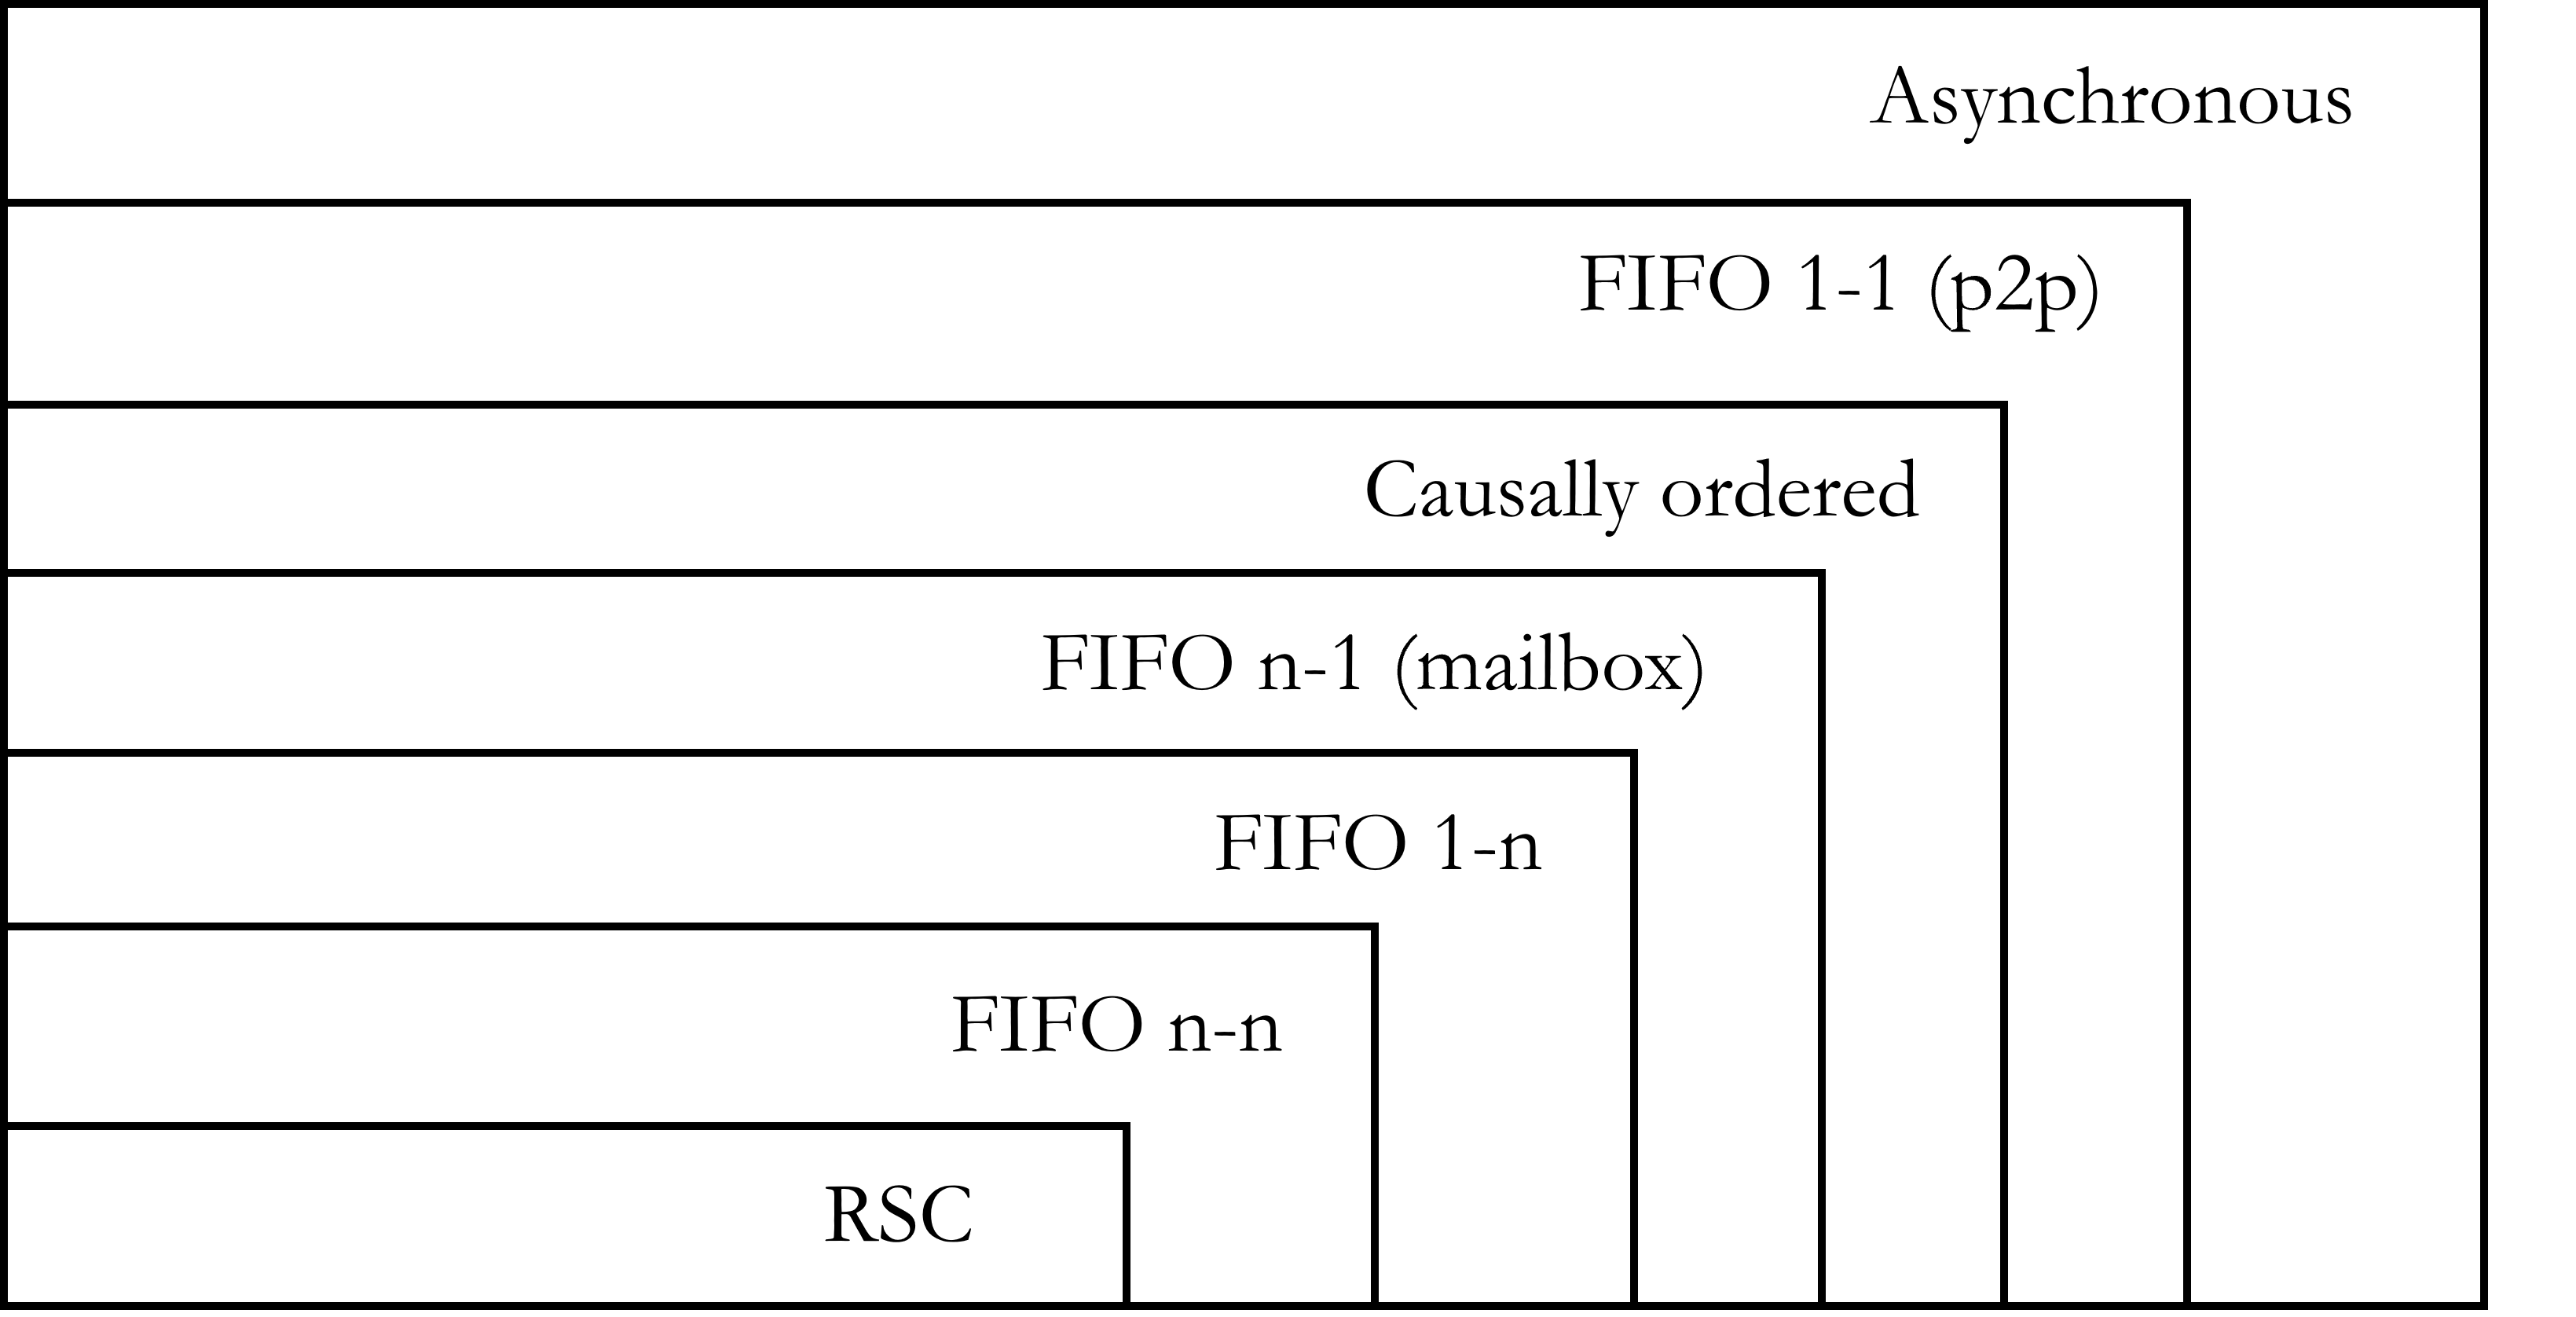
\includegraphics[width=10cm]{msc_hierarchy}
	\caption{The hierarchy of MSC classes.}
	\label{fig:msc_hierarchy_full}
\end{figure}